\documentclass[prb,preprint]{revtex4-1} 
% The line above defines the type of LaTeX document.
% Note that AJP uses the same style as Phys. Rev. B (prb).

\usepackage{amsmath}  % needed for \tfrac, \bmatrix, etc.
\usepackage{amsfonts} % needed for bold Greek, Fraktur, and blackboard bold
\usepackage{graphicx} % needed for figures
\usepackage{color}
\usepackage{ulem}
\usepackage{multirow}
\usepackage{gensymb}

\begin{document}

% Be sure to use the \title, \author, \affiliation, and \abstract macros
% to format your title page.  Don't use lower-level macros to  manually
% adjust the fonts and centering.

\title{Franck-Hertz Experiment}


\author{Liza Mulder}
\email{emulder@smith.edu}
\affiliation{Department of Physics, Smith College, Northampton, MA 01063}


\author{Frances Yang}
\email{fyang@smith.edu}
\affiliation{Department of Physics, Smith College, Northampton, MA 01063}


\date{\today}



\begin{abstract}
The Franck-Hertz experiment demonstrates the quantum mechanical nature of atoms: the energy levels are discrete. 
In this experiment, electrons are accelerated to increasing energies and sent through an atomic gas. The current of electrons reaching the cathode after converting to a voltage is measured. 
Since the atoms can only gain discrete amounts of energy, there will be dips in the current, corresponding to the electrons transferring energy to the atoms, subsequently unable to reach the cathode.
By looking at the spacing of dips in the data, one can determine the transition energies of the atom. 
We performed the Franck-Hertz experiment with neon and mercury gas, with the mercury at various temperatures. 
We also performed the experiment with mercury at 204\degree C using a lock-in amplifier by adding small sinusoidal oscillations on top of the relatively larger voltage used to accelerate the electrons.
We visually estimated the minima locations and uncertainties directly from the plots. 
This gave better results compared to using curve fits to determine the minima.
We obtained an estimate of $4.76\pm 0.03$ of the lowest excitation energy of mercury from our minima spacing data.
This lies between accepted values for the first two transition energies of mercury,  $4.67$ and $4.8$, but agrees with neither of them.
We think the discrepancy is caused by the lack of control in accelerating voltage, which made it difficult to accurately determine minima.
We think finer control of the accelerating voltage would allow us to collect more data, leading to more defined minima, allowing us to more accurately determine the lowest excitation energy of mercury. 
\end{abstract}

\maketitle

\section{Introduction} 

The Franck-Hertz Experiment is named for James Franck and Gustav Hertz, who used it to demonstrate discrete energy levels in atoms. 
They received the Nobel Prize in 1925 for their work on this experiment. 
In the experiment a beam of electrons is sent through a cloud of atoms, usually mercury or neon. 
Atoms can only gain energy in an amount equal to an allowed transition between energy levels. 
Only electrons with energies equal to these transition energies can transfer their energy to an atom. 
Electrons that have too much or too little energy will collide elastically with the atoms, keeping their energy. 
We find the transition energies by measuring the current of electrons leaving the gas - fewer reach the detector when they transfer energy to atoms in collisions. 
The loss in energy keeps those electrons from overcoming the retarding voltage at the anode. 
This causes dips (minima) in the current at voltages where many electrons can reach a transition energy one or more times during their journey through the gas. 
The spacing of the minima (in volts) gives the energy (in electron-volts) that colliding electrons gain between collisions - assuming the electrons lose all their energy in collisions. 
The next minimum occurs when the electrons gain back just enough energy to collide and lose their energy again. 
This energy gain - from zero to collision energy - is a transition energy of the atom. 
In this way the Franck-Hertz experiment can be used to determine the transition energies of the atom. 
Further research on the Franck-Hertz experiment in Mercury has shown a temperature dependence of the minima spacings, and examined how the minima spacings increase slightly at higher voltages. 
In our analysis we investigated temperature dependence briefly to chose a temperature at which the pattern in the data was most clearly defined, and we used the expected increase in minima spacing with voltage to better estimate the actual transition energy occuring in the gas. 


\section{Methods}

For this experiment we used a Franck-Hertz experimental apparatus from ELWE. A diagram is shown in Figure ~\ref{set-up}. 
First, we heat the oven containing the glass tube with mercury gas to the desired temperature. 
(In the diagram the part of the apparatus conatined in the oven is shaded grey.) 
Next, a filament with 120 mA of current creates a cloud of electrons inside the mercury gas. 
We set the filament voltage by placing an ammeter in line between the control box and the filament, then raising the filament voltage until the meter stabilized at 120mA. 
Inside the gas, a potential difference (which we call the accelerating voltage) drives the electrons through the apparatus. 
The voltage is applied to a grid inside the gas - it attracts the electrons but allows them to pass through it, eventually reaching the anode. 
We can control the energies of the electrons by varying the accelerating voltage. 
Electrons which have transferred energy in collisions have less energy at the other end of the apparatus, and a retarding potential prevents these electrons from reaching the anode. 
We set the retarding potential at 5V. %check this number
The current at the anode is converted to a voltage by the apparatus - the current runs through a resistor inside the control box, and the control box has an output which is the voltage across that resistor. 
This voltage is our output voltage. 
To take data, we slowly increased the accelerating voltage from zero until the gas began to ionize, and measured the output voltage from the anode. 

We performed this experiment with neon gas and mercury gas. 
The neon experiment yielded poor data: we could only discern two peaks, and their shapes were irregular. 
Therefore, we took the bulk of our data with mercury. 
The mercury gas experiment was performed with gas temperatures from 170\degree--210\degree C. 
Then was done so we could select an optimum temperature at which to take data with the lock-in. 
We decided on 204 \degree C. 

For direct measurements, we connected the accelerating voltage from the control box to a multimeter, and the output voltage to another multimeter. 
With the computer, we plotted accelerating voltage versus output voltage. 
The procedure for using the lock-in was more complicated. 
We used a function generator to add a periodic voltage on top of the accelerating voltage supplied by the control box. 
We then connected the reference from the function generator and the output voltage to the lock-in detector, and the resulting signal went to the second multimeter in place of the unmodified output voltage. 
Using the lock-in had the effect of taking the derivative of the orignal data - the minima locations changed, as did the shape of the peaks and dips. 
However, the spacing between the minima of the lock-in data had the same period as the original data: taking the derivative of a periodic funciton does not change its period. 
Therefore we used the minima spacing from both the direct data and the lock-in data to try and extract the transition energy. 

\begin{figure}[h!]
\centering
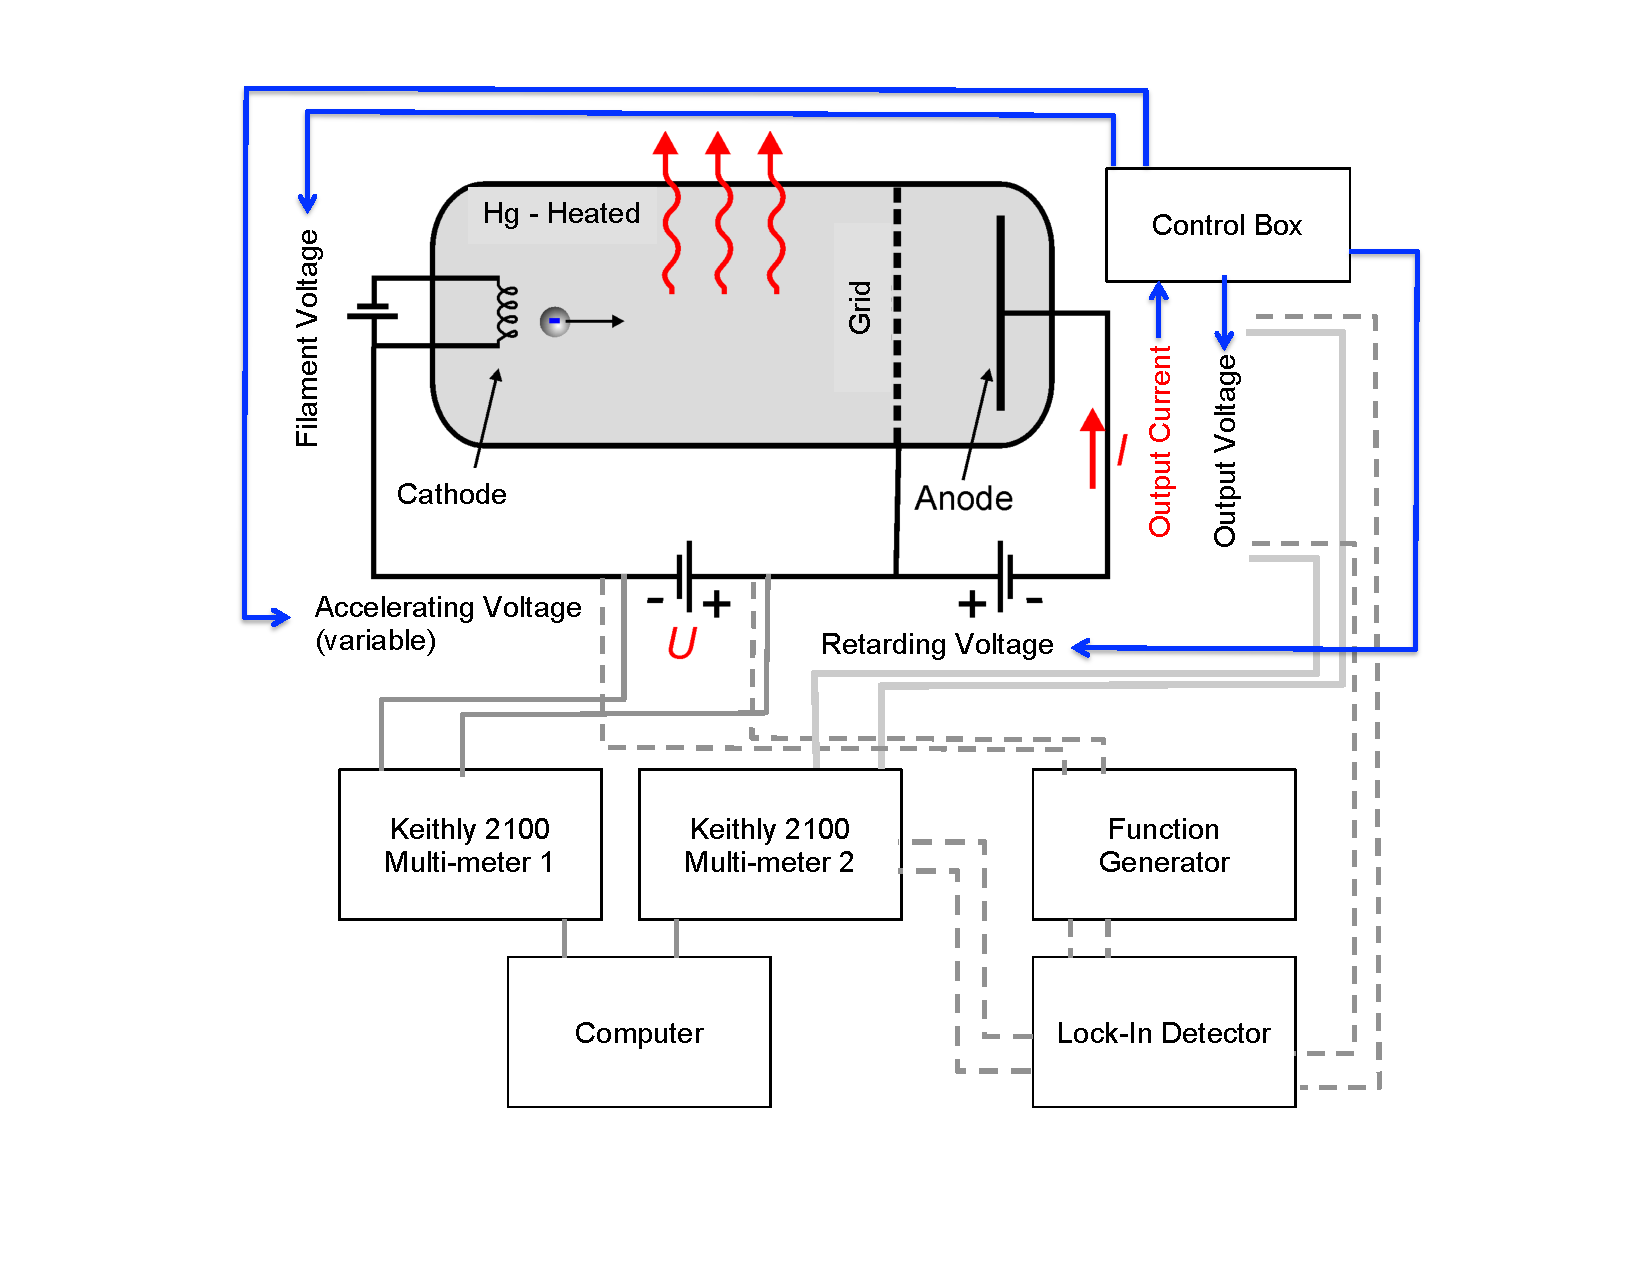
\includegraphics[width=5in]{set-up.pdf} %Shorten caption, write in procedure
\caption{The ELWE experimental apparatus, with the connections used to take measurements using both the direct method and the lock-in method. The apparatus consists of a control box (supplying the filament voltage, accelerating voltage, retarding voltage, and output voltage) and an oven, inside of which is the cloud of heated gas, the filament, the grid, and the anode. The solid lines, light and dark grey, show the instrument connections for direct measurements. The dark grey lines, dashed and solid, show the instrument connections for the lock-in measurements. }
\label{set-up}
\end{figure}

\section{Results}

Figure ~\ref{alltemps} shows our data for mercury gas at various temperatures. 
At lower temperatures, the output voltage values rose more quickly, and ionization voltage (where we stopped taking data) occured at lower values of accelerating voltage. 
At high temperatures the output voltage values rose slowly, so we could record more peaks before ionization, but the earlier peaks were shallower and less well defined. 

\begin{figure}[h!]
\centering
\includegraphics[width=6in]{alltemps.pdf}
\caption{A plot of the measured output voltage as a function of accelerating voltage for various temperatures of mercury gas. The general background trend flattens as the temperature increases.}
\label{alltemps}
\end{figure}


After comparing the curves, we decided that the data for 204 \degree C (the blue curve in Figure ~\ref{alltemps}) had the most minima without losing the first few to the decreasing amplitude. Figure ~\ref{204CbackFit} shows our data with a polynomial background fit. 

\begin{figure}[h!]
\centering
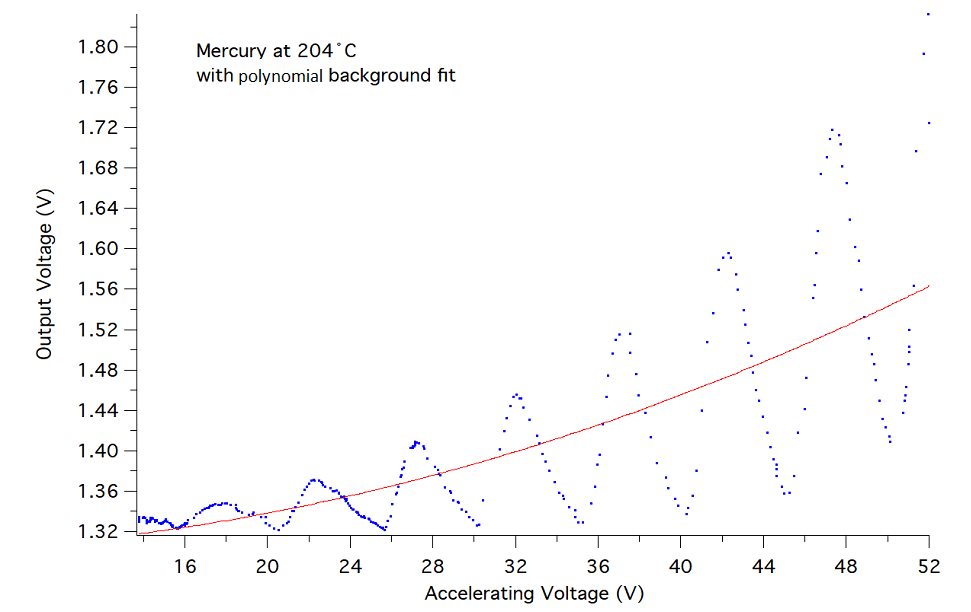
\includegraphics[width=6in]{204C_backFit.png}
\caption{A plot of the measured output voltage as a function of accelerating voltage for mercury gas at 204 \degree C. The general background trend is shown as a polynomial fit to the whole dataset.}
\label{204CbackFit}
\end{figure}

We also took data by the lock-in method, shown in Figure ~\ref{nobacklock} in the Analysis section with the background subtracted. 















































































































\section{Analysis}
Since we only saw two dips in our neon data, we did no further analysis it. Our mercury data was imported into Igor Pro. Most of our analysis was performed on data at 204\degree C. 
We first fit a background curve to both the data using the lock-in and the data without so it can be removed.
It is easier to determine the minima without the background present.
The curves were fitted using trial and error; we picked the one that best split the oscillations of the output voltage into equal amplitudes above and below the background. 
Fig. \ref{nobacknolock} and \ref{nobacklock} show the output voltage with the background removed. 

\begin{figure}[h!] %background not quadratic from my memory-fix
\centering
\includegraphics[width=6in]{204C_noback.png}
\caption{A plot of the output voltage minus the background for mercury at 204\degree C.}
\label{nobacknolock}
\end{figure}

\begin{figure}[h!]
\centering
\includegraphics[width=6in]{204C_lockin_noback.png}
\caption{A plot of the output voltage minus the background using the lock-in for mercury at 204\degree C}
\label{nobacklock}
\end{figure}

The minima for the data without the lock-in look parabolic while those of the lock-in data look linear.
We performed linear fits on each side of the minimum for the lock-in data. The intersection of these lines was our estimate of the minimum.
The curve fitting was done using Mathematica, as the uncertainties in the minima from curve-fitting in Igor Pro were larger than the range we fit the data over, thus they were not a accurate measure of our uncertainty in determining the minima.
We determined our uncertainty by first altering the slope and intercept of the best-fit line determined by Igor Pro, such that the line was no longer a good fit to the data. We obtained high and low values of the slope and intercept. 
Thus our uncertainty in the slope and intercept values was half of the difference between the high and low values.
Finally, the uncertainty in our minimum was determined by propagating the slope and intercept errors.
Although this method reduced the uncertainty relative to that from Igor Pro,  the range of values for each minimum was still larger than what it appears to be looking at the data. Additionally, some values of the minima did not appear to match when we compared it to our data by eye.
At this point, we decided to use the old-fashioned method of estimating our minimum by eye as well as the uncertainty for our both sets of data. Then we calculated the spacing between successive minima (Table ~\ref{minimaSpacing} and Fig. \ref{nomineye}). 

The spacings should increase linearly with the number of minima, due to extra acceleration of the electron before it collides with an atom. The expected spacing between minima is given by 
\begin{equation}\label{energy}\Delta E(n)=E_n-E_{n-1}=\left\lfloor 1+\lambda/L(2n-1)\right\rfloor E_a,\end{equation}
where $\lambda$ is the mean free path of the electron (the average distance it moves before colliding), $L$ is the anode to cathode distance, and $E_a$ is the lowest excitation energy of the atom. The lowest possible excitation energy from Eq.~\ref{energy} is $E_a=\Delta E(0.5)$. \cite{new}
We can obtain a estimate of the lowest excitation energy of mercury by extrapolating our linear fit of data in Table~\ref{minimaSpacing} to $n=0.5$. 

\begin{table}[h!]
\centering

\caption{Values for minima spacing with uncertainty, determined by three methods: estimating by eye from the plot of lock-in data, estimating by eye from the plot of data taken without the lock-in, and calculating from the curve fits to the lock-in minima as described in the analysis section. Our eyeball estimates had the lowest uncertainty. The estimate by eye of the data without lock-in (columns 4 and 5 in the table) is plotted in Figure ~\ref{nomineye}}

\begin{ruledtabular}
\begin{tabular}{cccccccl}
          & \multicolumn{2}{l}{\begin{tabular}[c]{@{}l@{}}Lock-in data\\ estimate by eye\end{tabular}} & \multicolumn{2}{l}{\begin{tabular}[c]{@{}l@{}}Data without lock-in\\ estimate by eye\end{tabular}} & \multicolumn{2}{l}{\begin{tabular}[c]{@{}l@{}}Lock-in data\\ calculated from fits\end{tabular}} \\
n & X                                            & dX                                          & X                                                & dX                                              & X                                              & dX                                             \\
1         & 4.87                                         & 0.2                                         & 4.82                                             & 0.12                                            & 5                                              & 0.9                                            \\
2         & 5.15                                         & 0.2                                         & 4.79                                             & 0.14                                            & 5.07                                           & 0.53                                           \\
3         & 4.5                                          & 0.2                                         & 4.91                                             & 0.12                                            & 4.49                                           & 0.43                                           \\
4         & 5.1                                          & 0.2                                         & 4.95                                             & 0.15                                            & 5.11                                           & 0.43                                           \\
5         & 4.9                                          & 0.2                                         & 5                                                & 0.3                                             & 5.01                                           & 0.43                                           \\
6         & 4.95                                         & 0.2                                         & 5.2                                              & 0.35                                            & 4.89                                           & 0.4                                            \\
7         & 5.31                                         & 0.25                                        & 5.13                                             & 0.22                                            & 5.29                                           & 0.46                                          
\end{tabular}
\end{ruledtabular}
\label{minimaSpacing}
\end{table}

\begin{figure}[h!]
\centering
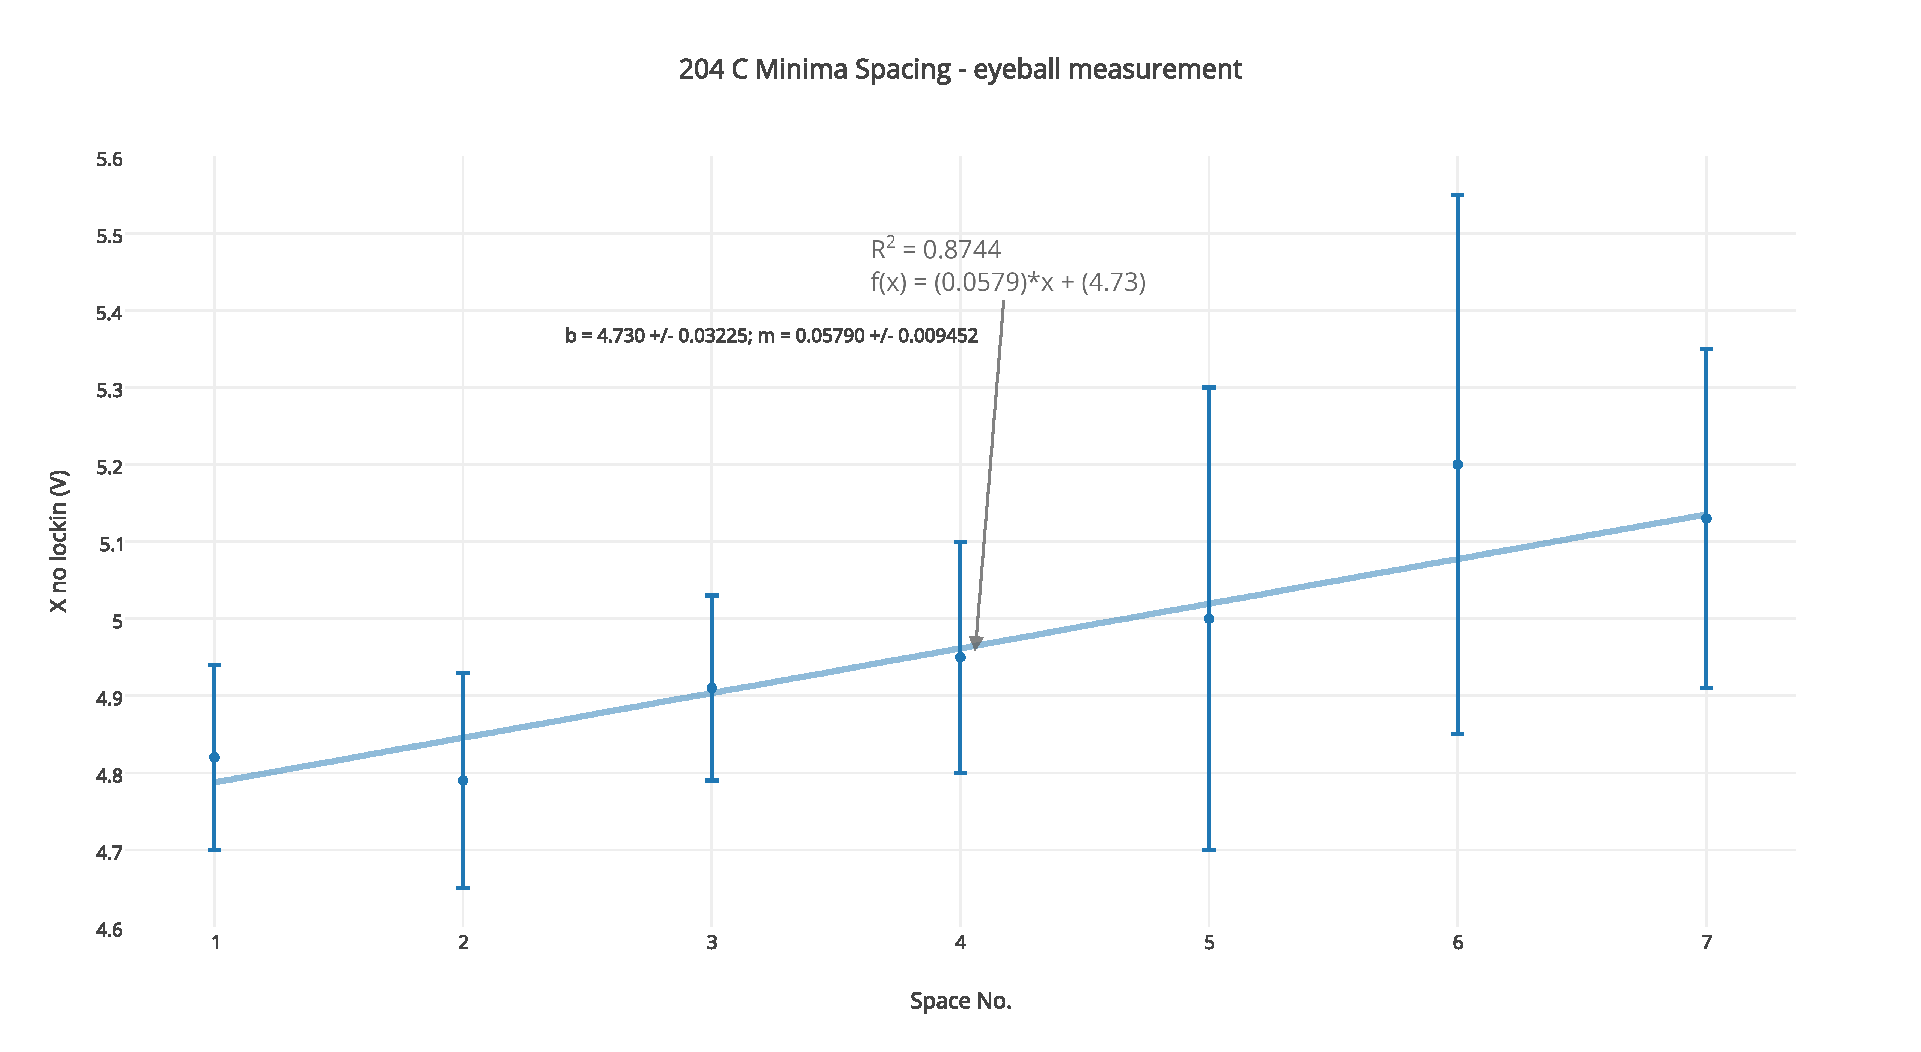
\includegraphics[width=6in]{204C_minima_eyeball.pdf}
\caption{A plot the change in accelerating voltage between successive minima.}
\label{nomineye}
\end{figure}

We estimated the lowest excitation energy of mercury to be $4.76\pm0.03$
from the minima of the lock-in data estimated by eye, of the no lock-in data estimated by eye, and of the lock-in data estimated by curve-fitting.


\section{Discussion}










\section{Conclusion}


\begin{thebibliography}{3}

\bibitem{new} Gerald Rapior, Klaus Sengstock, and Valery Baev, "New features of the Franck-Hertz experiment," Am. J. Phys. {\bf 74}, 423--428 (2006).

\end{thebibliography}
\end{document}
